\begin{figure}
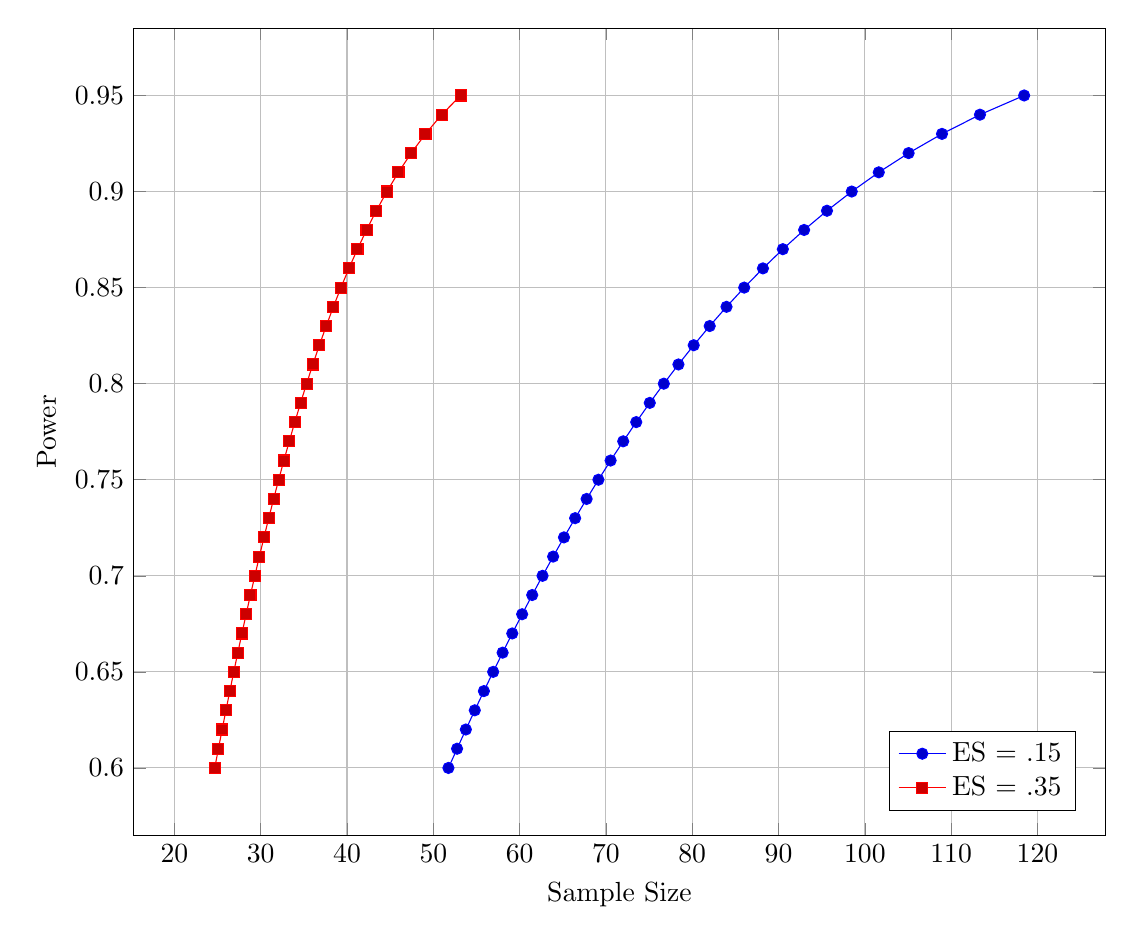
\begin{tikzpicture}
	\begin{axis}[grid=major,xlabel=Sample Size,ylabel=Power,scale=1.8, legend pos= south east] 
\addplot coordinates{
(51.7495	,0.60)
(52.7503,	0.61)
(53.7678,	0.62)
(54.8031,	0.63)
(55.8574,	0.64)
(56.9318,0.65)
(58.0275,	0.66)
(59.1461,	0.67)
(60.289,	0.68)
(61.4578,	0.69)
(62.6543,	0.70)
(63.8806,	0.71)
(65.1387,	0.72)
(66.4311,	0.73)
(67.7605,	0.74)
(69.1297,	0.75)
(70.5422,	0.76)
(72.0015,	0.77)
(73.512,	0.78)
(75.0783,	0.79)
(76.7058,	0.80)
(78.4009,	0.81)
(80.1708,	0.82)
(82.0239,	0.83)
(83.9701,	0.84)
(86.0213,	0.85)
(88.1917,	0.86)
(90.4986,	0.87)
(92.9634,	0.88)
(95.6129,	0.89)
(98.4816,	0.90)
(101.614,	0.91)
(105.072,	0.92)
(108.939,	0.93)
(113.339,	0.94)
(118.46	,0.95)};
\addlegendentry{ES = .15}

\addplot coordinates{
(24.6688	,0.60)
(25.095,	0.61)
(25.5284,	0.62)
(25.9694,	0.63)
(26.4186,	0.64)
(26.8765,	0.65)
(27.3435,	0.66)
(27.8203,	0.67)
(28.3075,	0.68)
(28.8059,	0.69)
(29.3161,	0.70)
(29.8392,	0.71)
(30.3758,	0.72)
(30.9272,	0.73)
(31.4944,	0.74)
(32.0787,	0.75)
(32.6815,	0.76)
(33.3044,	0.77)
(33.9492,	0.78)
(34.6179,	0.79)
(35.3129,	0.80)
(36.0368,	0.81)
(36.7927,	0.82)
(37.5842,	0.83)
(38.4156,	0.84)
(39.292,	0.85)
(40.2194,	0.86)
(41.2052,	0.87)
(42.2586,	0.88)
(43.3911,	0.89)
(44.6174,	0.90)
(45.9568,	0.91)
(47.4353,	0.92)
(49.089,	0.93)
(50.9706,	0.94)
(53.1614,	0.95)};
\addlegendentry{ES = .35}


\end{axis}
\end{tikzpicture}
\caption[Time Variables Power Graph]{Time Variables Power Graph}
\label{fig:TVPowerGraph}
\end{figure}